\documentclass[11pt]{ctexart}
\usepackage[margin=2.3cm]{geometry}
\usepackage{graphicx}
\usepackage{booktabs}
\usepackage{amsmath}
\usepackage{amssymb}
\usepackage{xcolor}
\usepackage{caption}
\usepackage{mdframed}
\usepackage[colorlinks=true,linkcolor=blue!60!black,urlcolor=blue!60!black]{hyperref}

\definecolor{good}{HTML}{2E7D46}
\definecolor{bad}{HTML}{B23B3B}
\definecolor{warn}{HTML}{9A6A00}
\newcommand{\cmd}[1]{\texttt{\small #1}}
\newcommand{\yes}{\textcolor{good}{\textbf{是}}}
\newcommand{\no}{\textcolor{bad}{\textbf{否}}}
\captionsetup{font=small}

\title{\bfseries 32 导干电极脑电帽\\运动想象(MI)初期测试报告}
\author{EEG\_MI 项目}
\date{2026 年 7 月 27 日}

\begin{document}
\maketitle

\begin{abstract}
\noindent
三次真实采集(共 155 个 trial)后的阶段性结论:\textbf{采集链路已达到可用水平}(稳态丢包
0.000\%,时序精度 8.96\,s/trial,全通道无损保存);\textbf{左右手想象不可分}(置换检验
$p=0.41$);\textbf{"做任务 vs 休息"可分}(多种方法稳定在 0.83–0.87);\textbf{手 vs 脚在 mu 频段
可分}($\mathrm{AUC}=0.704$, $p=0.040$)——但后者需要\textbf{剔除无效通道并选对频段}才能显现,
用默认全通道流水线会被淹没。横向测评 \textbf{7 个} EEG foundation model(含新接入的 EEGPT/BENDR/BIOT/SignalJEPA),
冻结表征\textbf{全部劣于}经典 Riemannian/带功率方法,且模型规模不预测表现。报告同时记录一个不可忽视的混淆:受试无 MI 经验,主观上\textbf{"抑制真实
动作"的心理活动强于运动想象本身},本数据无法区分二者。
\end{abstract}

\section{采集质量:已达可用水平}
三次会话的链路指标(全部为 32 导全通道保存,无任何通道筛选):

\begin{center}\small
\begin{tabular}{@{}lrrrrl@{}}
\toprule
会话 & trial & 时长 & 丢包 & 重建样本 & 备注 \\
\midrule
左手/右手      & 30 & 270\,s & 0.108\,\% & 0 & 完整 \\
双手/休息      & 50 & 170\,s & 0.308\,\% & 0 & \textcolor{bad}{数据流中断,仅 19 个有效} \\
手/脚/减7      & 75 & 675\,s & 0.045\,\% & 0 & \textcolor{good}{75/75 全有效,0 次中断} \\
\bottomrule
\end{tabular}
\end{center}

第二次会话在约 170\,s 处采样流静默中断,后 31 个 trial 被记录在同一个(无意义的)样本位置。
根因是接收 socket 没有超时,板子停发后线程永久阻塞——界面看起来"卡住"却无任何报错。修复后
(2\,s 超时 + 自动重发初始化 + 范式自动中止)第三次会话 \textbf{75/75 全部有效}。

另有两个已确认的硬件问题:\textbf{F7 为间歇性开路}(连续四次会话恒定在 $+187500\,\mu$V 满量程、
唯一值仅 1 个 = 输入浮空;而在 SSVEP 测试中又正常——是接插件/导线的间歇断路,不是头皮接触);
\textbf{FC1 接触极差}(有慢漂移但 1–40\,Hz 内容为 0)。

\section{方法}
每份录制都做了\textbf{广度搜索}而非单一流水线:4 种通道集 $\times$ 5 个频段 $\times$ 6 种特征/分类器
= 115 个组合,外加 \textbf{7 个}冻结 foundation model 的 embedding 线性探针。评估用 5 折 $\times$ 多次重复
分层交叉验证;\textbf{最终结论只采信置换检验}。个体 mu 峰实测在 \textbf{7.0\,Hz}(低于教科书的
10–12\,Hz),故频段扫描包含 6–9\,Hz。

\section{结果}

\subsection{左手 vs 右手:不可分}
$\mathrm{AUC}=0.60$,置换检验 $p=0.41$。ERD 方向亦不对(左手 contra C4 $+3\%$、ipsi C3 $-4\%$)。
全场唯一显著的效应在\textbf{枕区} 13–30\,Hz($+46\%$, $p=0.023$)——是提示屏驱动视觉皮层,不是运动。
该会话的倒计时数字在想象期内变化 4 次,每次都是一个视觉瞬变;已改为想象期画面静止。

\textbf{解读:}左右手需要区分 C3 与 C4 的精细侧化,这超出了干电极帽的空间分辨能力。

\subsection{双手 vs 休息:可分且稳健}
115 个组合中\textbf{最好 0.867、最差 0.361},且 0.80 以上的组合广泛分布于不同通道集与频段——
这种\emph{跨方法的一致性}比单一的高分更有说服力。独立的 ERD 证据同向:感觉运动区
8–13\,Hz 双手 $-24.9\%$($p=0.007$)、休息 $+36.8\%$($p=0.012$),\textbf{两者方向相反}(图~\ref{fig:erd})。

\begin{figure}[h]\centering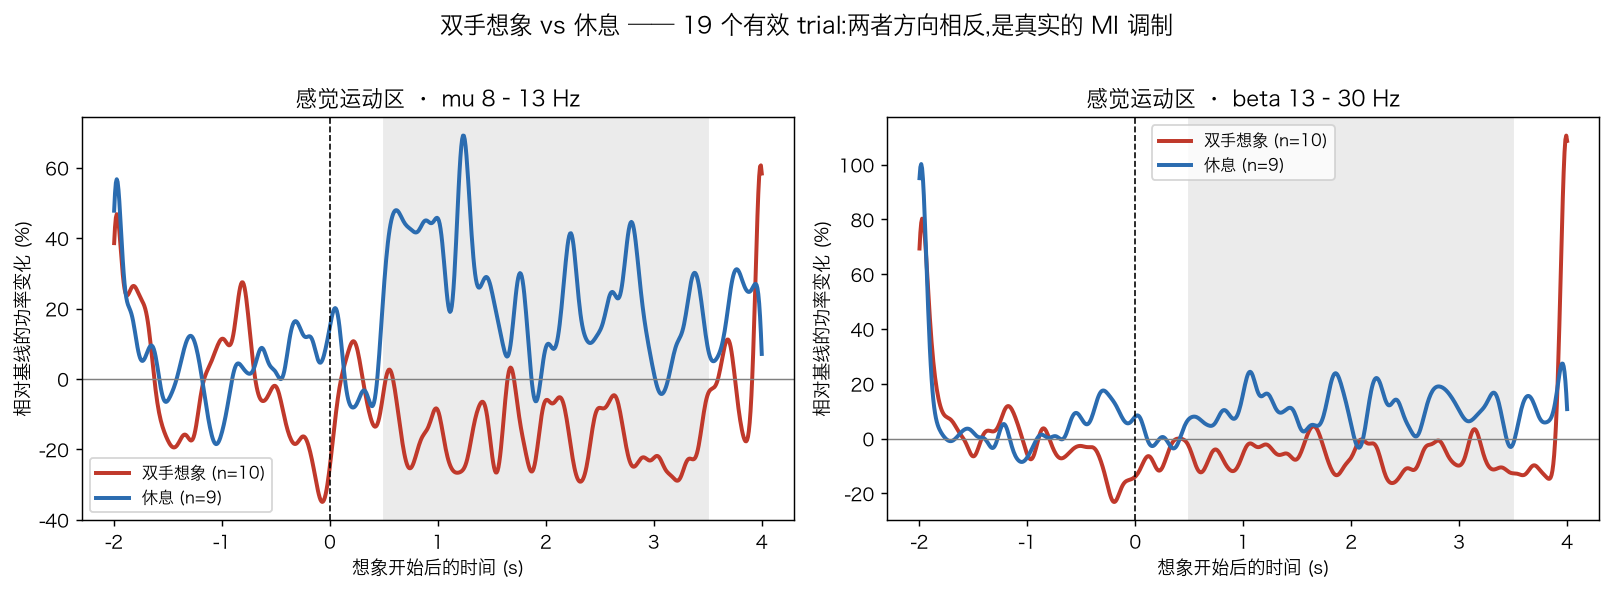
\includegraphics[width=\linewidth]{hands_rest_erd.png}
\caption{双手想象(红)与休息(蓝)在感觉运动区的功率变化,分居零线两侧。仅 19 个有效 trial。}
\label{fig:erd}\end{figure}

\begin{mdframed}[linecolor=warn,backgroundcolor=warn!5]
\textbf{必要的自我修正:}早先报告过该对比"$\mathrm{AUC}=0.90$, $p=0.024$"。那是 $n=19$、且在扫过
5 个频段后挑最好的一个做的置换检验,\textbf{偏乐观}。本次广度搜索给出的 0.83–0.87 更可信。
\end{mdframed}

\subsection{手/脚/减7 三分类:整体接近随机,但存在真实的局部结构}
三分类准确率最好 0.480(随机 0.333),置换 $p=0.010$——但这是 115 个组合中选出的最好值,$p$ 值
本身偏乐观。逐通道比较三个任务的 ERD 地形,显著差异的通道数为 0/32、1/32、2/32(随机期望
$\approx$1.6),即\textbf{用默认全通道流水线看,三个任务的空间模式几乎一样}。

\textbf{但换一种切法就不同了。}限定到\textbf{中央+额区 17 导}(剔除已知坏道)并用 \textbf{mu 8–13\,Hz}:

\begin{center}\small
\begin{tabular}{@{}lccc@{}}
\toprule
对比 & mu 8–13 & beta 13–30 & wide 4–40 \\
\midrule
\textbf{手 vs 脚} & \textcolor{good}{\textbf{0.704}}$^{*}$ & 0.605 & 0.571 \\
运动(手+脚) vs 心算 & 0.474 & 0.595 & 0.638 \\
手 vs 心算 & 0.598 & 0.573 & 0.514 \\
\bottomrule
\end{tabular}
\end{center}
\noindent {\small $^{*}$ 置换检验 $\mathrm{AUC}=0.704$,随机均值 0.512,\textbf{$p=0.040$},$n=50$。}

\textbf{手 vs 脚在 mu 频段确实可分},且符合躯体定位学(手在外侧 C3/C4、脚在内侧 Cz)。这修正了
"三个任务无差异"的早期结论——差异存在,只是被无效通道和错误频段淹没了。\textbf{通道选择是关键}。

\subsection{Foundation model:七个预训练模型的横向测评}
共测试 \textbf{7 个} EEG foundation model 的\textbf{冻结}表征 + 线性探针。五个来自 braindecode 1.6
的官方 HuggingFace 权重(本次新增,含此前一直无法获取的 \textbf{EEGPT}),两个是项目里已有的本地权重。

\paragraph{接入方法。}每个 checkpoint 的预训练 montage 与采样率都不同,32 导干电极帽无法直接喂入:
\begin{itemize}
\item \textbf{通道}:checkpoint 自带具名 montage 的(EEGPT 62 导、LaBraM 128 导、SignalJEPA 62 导、
      BENDR 20 导),按\textbf{导联名}把我们的电极放进对应位置,\textbf{其余置零}——不做插值、不伪造信号;
      只固定通道\emph{数}的(BIOT 18 导)走 braindecode 的 \cmd{Interpolated*} 样条插值。
      BENDR 的固定表用旧命名 T5/T6,已映射到我们的 P7/P8。
\item \textbf{采样率/长度}:重采样到 checkpoint 的 sfreq 并裁剪/补齐到其 n\_times。
\item 分类头替换为 Identity,取\textbf{倒数第二层}表征;高维 embedding 先 PCA 降到 $\le n/3$ 维,
      避免 $n \ll d$ 时线性探针靠记忆刷分。
\end{itemize}

\begin{center}\small
\begin{tabular}{@{}lrrcc@{}}
\toprule
模型 & 参数 & embedding 维 & 双手/休息(随机 .500) & 三分类(随机 .333) \\
\midrule
\textbf{[经典] TS+LR mu} & — & — & \textbf{0.790} $\pm$.19 & 0.365 $\pm$.10 \\
\midrule
BENDR        & 157.1\,M & 512    & \underline{0.733} $\pm$.22 & \textbf{0.392} $\pm$.10 \\
BIOT         & 3.2\,M   & 256    & 0.703 $\pm$.20 & 0.253 $\pm$.07 \\
EEGPT        & 25.3\,M  & 63\,488 & 0.673 $\pm$.19 & \underline{0.373} $\pm$.10 \\
CBraMod(本地) & 4.0\,M  & 6\,200 & 0.700 $\pm$.18 & 0.298 $\pm$.11 \\
SignalJEPA   & 3.5\,M   & 27\,776 & 0.597 $\pm$.21 & 0.336 $\pm$.09 \\
LaBraM(本地) & 5.8\,M   & 6\,200 & 0.589 $\pm$.27 & 0.262 $\pm$.09 \\
LaBraM(官方) & 5.8\,M   & 200    & 0.503 $\pm$.21 & 0.309 $\pm$.10 \\
\bottomrule
\end{tabular}
\end{center}

\paragraph{结论。}
\begin{enumerate}
\item \textbf{没有任何冻结 FM 超过经典流水线}。在信号确实存在的双手/休息上,经典 TS+LR 取得 0.790,
      最好的 FM(BENDR)只有 0.733;在三分类上所有方法都贴着随机线,名义最好的 BENDR 0.392 其
      标准差就有 0.099。
\item \textbf{模型规模不预测表现}。BENDR 有 157\,M 参数(比 BIOT 大 49 倍),优势却只有 3 个百分点;
      3.2\,M 的 BIOT 在双手/休息上反超 25.3\,M 的 EEGPT。
\item \textbf{官方 LaBraM 权重在二分类上恰好等于随机}(0.503)。同一架构的本地权重是 0.589——
      说明差异来自预训练数据/权重版本,而非架构。
\item 这与我们在公开数据 BCI IV-2a 上的结论完全一致:\textbf{冻结的通用 backbone 无法线性暴露 MI
      所需的细微空间对比},要有竞争力必须微调。
\end{enumerate}

\paragraph{一个必须说明的技术细节。}EEGPT 的 \cmd{chan\_proj\_type} 默认会\textbf{强制把任意输入投影到
它自己的 19 导标准集}并忽略传入的 montage,导致 62 导 checkpoint 加载失败;必须显式指定
\cmd{chan\_proj\_type="none"}。这类"默认参数与 checkpoint 不匹配"的坑在跨模型比较里很容易造成
"某模型不行"的错误结论——本次五个模型里有三个需要各自的加载修正才跑得起来。

embedding 空间的直接可视化(图~\ref{fig:emb})也印证了数值:三分类在任何特征空间里都没有可见聚类。

\begin{figure}[h]\centering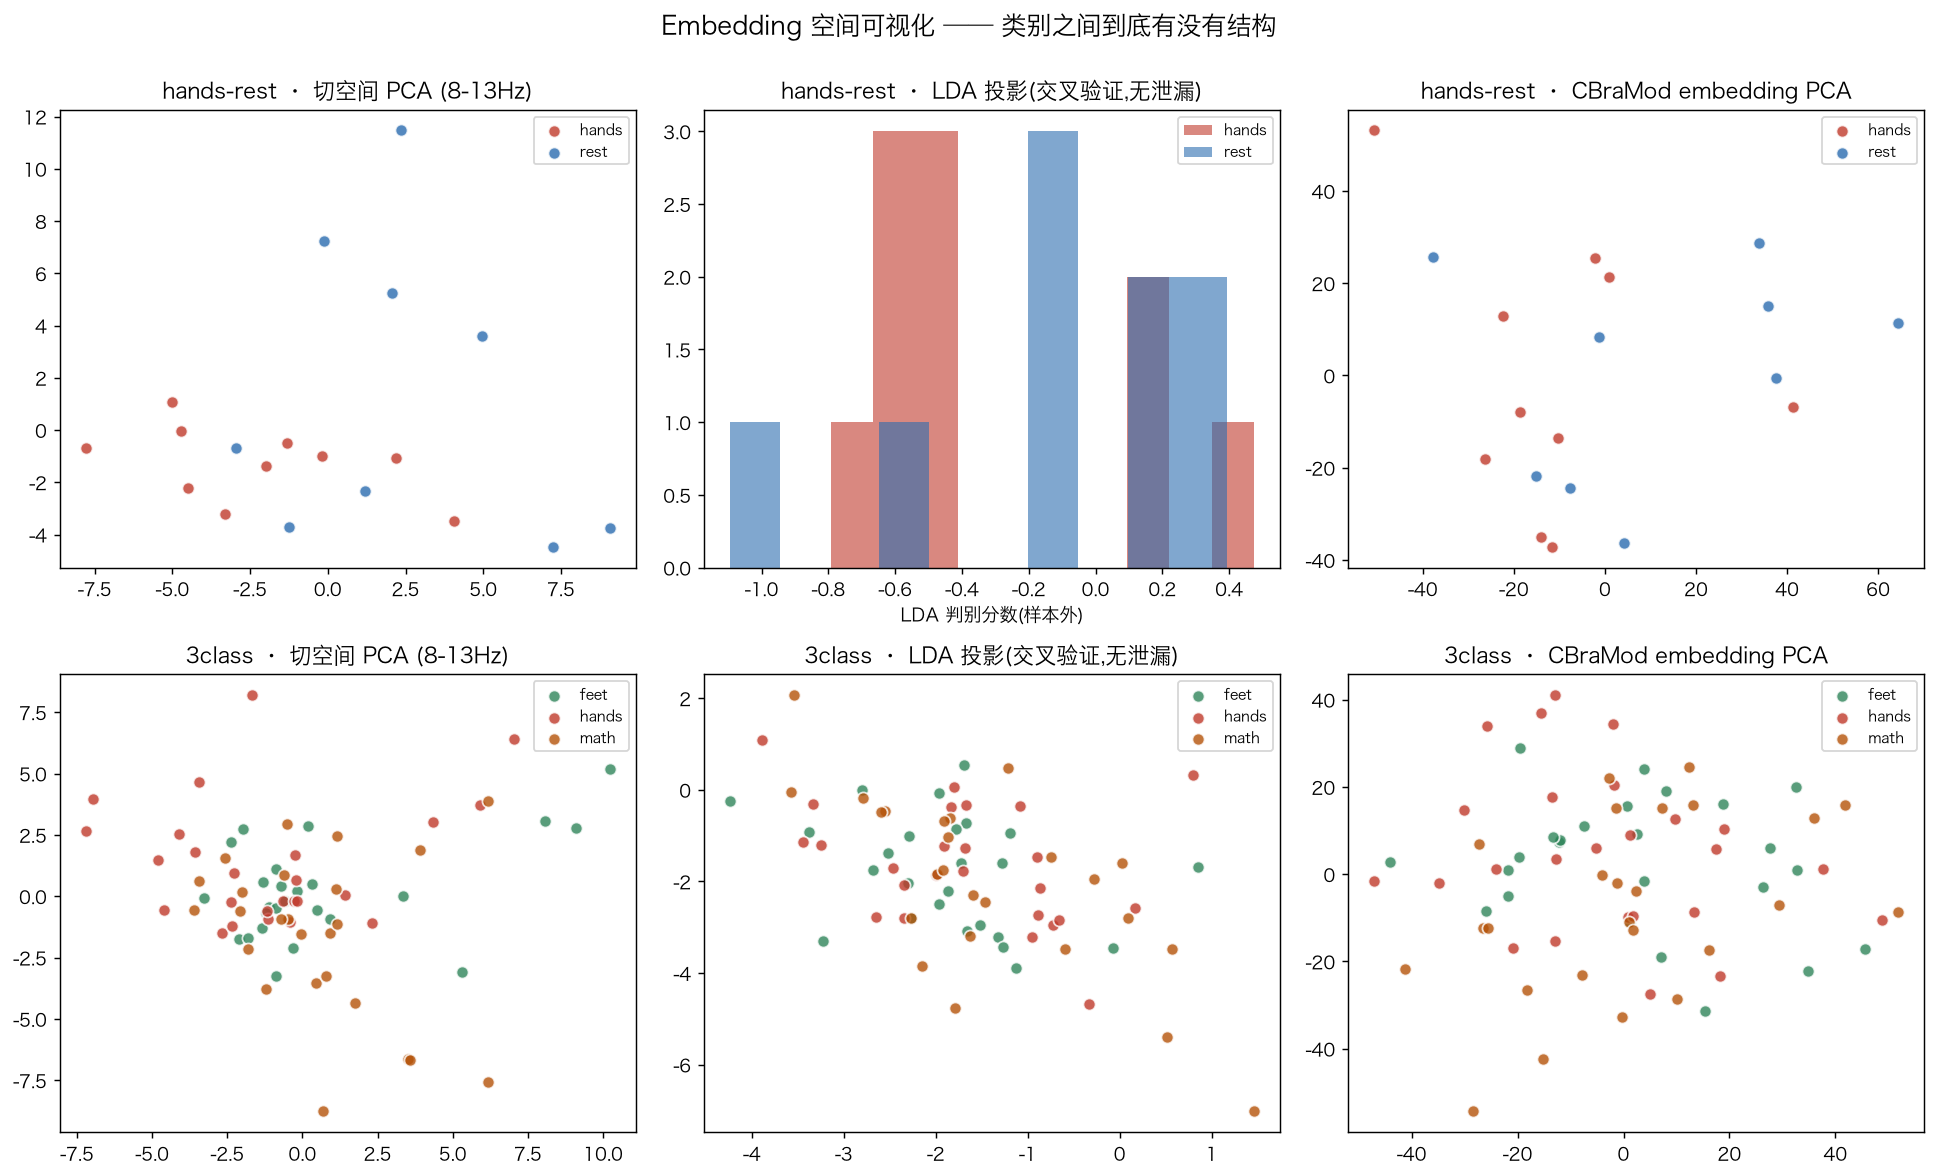
\includegraphics[width=\linewidth]{embedding_explore.png}
\caption{切空间 PCA、交叉验证 LDA 投影(无泄漏)、CBraMod embedding PCA。上排 hands/rest 可见
部分分离,下排三分类无可见结构。}
\label{fig:emb}\end{figure}

\section{关键混淆:抑制动作 vs 运动想象}
受试报告:因无 MI 经验,任务中\textbf{"压住不要真的动"的心理活动明显强于运动想象本身}。
这是一个必须记录的混淆——本数据\textbf{无法区分二者},原因是:

\begin{itemize}
\item 运动抑制与运动想象\textbf{都会调动感觉运动网络},且\textbf{都具有躯体定位组织}——
      "抑制手"与"抑制脚"同样会产生 C3/C4 与 Cz 的差异。因此 0.704 这个手/脚可分的结果,
      对两种解释同样成立。
\item 二者对 beta 的作用\textbf{方向相反}(抑制倾向于升高 beta,想象倾向于降低),会部分抵消——
      这与我们观察到的 beta ERD 微弱且不稳定($-10\%\sim-20\%$,时显时不显)相符。
\item 一个简单的预测——"若抑制主导,则两个运动类彼此难分"——\textbf{未被支持}(手 vs 脚反而是
      最好分的对比)。所以不能简单地说"全是抑制"。
\end{itemize}

\noindent\textbf{对 BCI 而言影响有限}(无论是想象还是抑制,只要产生稳定可分的模式即可用),
\textbf{但对实验措辞和疲劳度影响很大}:持续抑制是费力的,可能是 7\,Hz 低频峰(困倦迹象)与
后半段表现下滑的原因之一。

\section{方法学诚实性说明}
\begin{enumerate}
\item \textbf{多重比较:}每个数据集搜索了 115 个组合。表中的"最好"值必然偏乐观;只有经过置换
      检验的结论(手 vs 脚 $p=0.040$;三分类 $p=0.010$)才具备统计意义,且后者仍受选择偏倚影响。
\item \textbf{样本量:}有效 trial 19–75 个。效应量 $d\approx1.0$ 时,80\% 检验效能需每类 $\approx$16–17
      个 trial;19 个 trial 的双手/休息刚好在边缘。
\item \textbf{单被试单会话:}所有结论仅对该受试、该次佩戴成立,不能外推。
\item \textbf{未做跨会话验证:}真正的"免重训"目标需要"前几天训练、后一天测试"的验证,尚未进行。
\end{enumerate}

\section{结论与下一步}
\textbf{已确立:}(1) 采集链路可靠;(2) "做任务 vs 休息"是当前最稳的二元对比;
(3) 手 vs 脚在 mu 频段存在真实的躯体定位差异,\textbf{前提是剔除无效通道并选对频段};
(4) 左右手在本硬件上不可行;(5) 冻结 FM embedding 不如经典方法。

\textbf{建议顺序:}
\begin{enumerate}
\item \textbf{修好 F7}(摇动测试 + 换位测试定位间歇断路),压好 FC1;
\item \textbf{重采双手/休息},每类 25 个 trial,验证 0.83–0.87 是否站得住;
\item \textbf{重采手 vs 脚},每类 30 个 trial,\textbf{预注册}分析方案(中央+额区、mu 8–13\,Hz、
      TS+LR),用"先注册后检验"消除选择偏倚——这是把 0.704 变成可信结论的唯一途径;
\item 调整指导语,降低"抑制"负担(例如明确告知"不用担心会真的动,专注在感觉上");
\item 若 2–3 成立,再考虑三分类与 FM 微调;若不成立,SSVEP 路线的信噪比要高一个量级。
\end{enumerate}

\vspace{0.6em}\noindent\rule{\linewidth}{0.4pt}\\[2pt]
{\small 复现:\cmd{python src/analysis/explore\_embeddings.py -{}-dataset both}。
原始数据全部为 32 导全通道保存于 \cmd{recordings/},分析中的通道剔除只作用于副本。}

\end{document}
